\noindent \textit{\textcolor{red!60!black}{
2. Broader macro story, of just large firms?\\ 
Only the largest firms in the economy issued bonds. In fact, more than ¼ but less than ½ of the firms in the sample had gold-denominated bonds. Was this a more general issue in the economy at large, for firms or households? If yes, it would be great to provide some descriptive evidence. If not, it shapes how we see the contribution of the paper to our understanding of the Depression. Yes, understanding large firm behavior is important, but the macro estimates in the latest section of the paper could not be extrapolated to the rest of the economy, making the effects of this channel on the very sizable contraction in private non-residential fixed investment much smaller.
}}

\bigskip

\noindent We thank you very much for this insightful comment. You are correct to point out that, in our original submission, we were not adequately discussing the relevance of our findings to the broader economy. In the revised manuscript, we address this issue in three places: (i) the ``Historical background'' section, (ii) the ``Aggregation'' section, and (iii) the ``Conclusion.''

First, we now discuss in the ``Historical background'' section how the issue of gold clauses was understood to extend beyond industrial firms at the time. We quote President Hoover's 1932 campaign speech in which he warned that ``A considerable part of farm mortgages, most of our industrial and all of our Government, most of our State and municipal bonds, and most other long-term obligations are written as payable in gold.'' We also include his warning to farmers that, if the US had gone off gold, they ``would have sold their produce for depreciated currency... but you would have to pay a premium on such of your debts as are written in gold.'' Given that agriculture employed nearly a quarter of the workforce at the onset of the Depression, the prevalence of gold clauses in farm mortgages underscores the broader economic relevance of the abrogation.

Second, in the ``Aggregation'' section, we now explicitly interpret our results as providing a lower bound for the total effect of gold clause abrogation on private investment:
\begin{quotation}
Finally, we interpret our aggregation results as providing a lower bound for the total effect of gold clause abrogation on private investment. As previously discussed, gold clauses were prevalent in other private contracts, including farm mortgages, public utility bonds, and railroad securities. The coverage of our data does not allow us to study the effects of the abrogation on these other borrowers, but our results suggest that the abrogation may have had economically significant effects on these sectors as well, which is an interesting avenue for future research.
\end{quotation}

Third, the ``Conclusion'' now identifies other sectors where the gold clause was prevalent as promising avenues for future research:
\begin{quotation}
While this paper focuses on the impact of gold clause abrogation on large industrial firms, examining its effects on other sectors of the economy represents a promising avenue for future research. Evidence suggests that gold clauses were prevalent in farm mortgages, making the agricultural sector a particularly important case for investigation. Given that agriculture employed nearly a quarter of the workforce at the onset of the Depression, understanding how the abrogation affected farmers' debt burdens, investment decisions, and recovery patterns could provide crucial insights into the policy's broader economic impact. Similarly, public utilities and railroads---major issuers of gold-denominated corporate bonds and critical components of economic infrastructure---warrant further attention.
\end{quotation}

An inspection of the Moody's Steam Railroads Manuals and the Moody's Public Utilities Manuals reveals that firms in these industries were large issuers of gold-denominated corporate bonds. We have excluded these firms from our analysis, because they were heavily regulated and very few were publicly listed which makes it difficult to measure their average Q and implement standard investment regressions. Nonetheless, we believe that examining the impact of the gold clause on these industries---as well as on agricultural investment---represents a promising avenue for future research.

\bigskip

\begin{figure}[h]
  \centering
  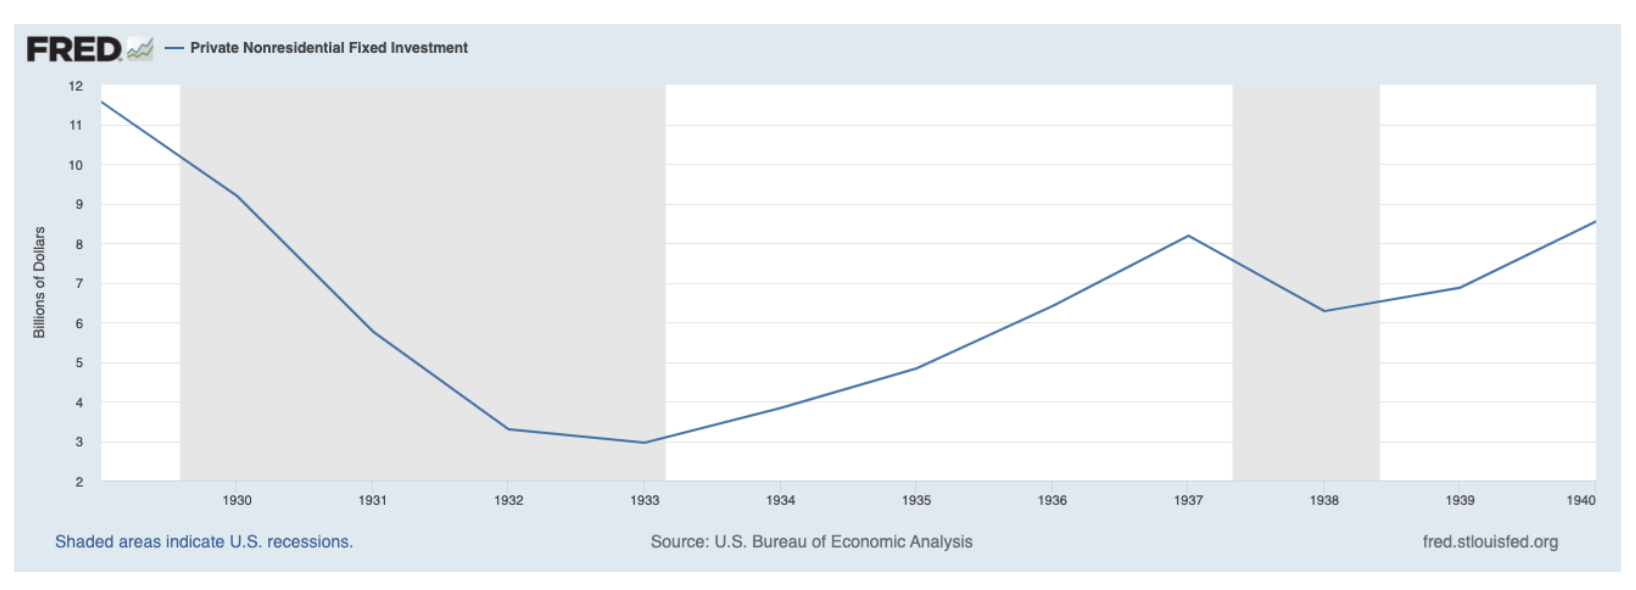
\includegraphics[width=\textwidth]{../../referee-responses-figures/r6-private-non-res-investment.png}
  \caption{Private non-residential investment}
  \label{fig:R6_private_non_res_investment}
\end{figure}

\textit{\textcolor{red!60!black}{
As shown above, most of the contraction in private fixed investment took place before 1932. Again, though the allocation within firms is significant, stating that "Taken together, our partial equilibrium aggregation exercise suggests that the uncertainty surrounding the abrogation of gold clauses led to a steep decline in public firms' investment and, therefore, likely contributed to the slow speed of economic recovery from the Great Depression. We find that leverage risk led public firms to delay investment in fixed capital for two years. This finding complements existing explanations of the delayed recovery based on the disruption of credit intermediation, which is more applicable to smaller firms. " seems much too strong, and the last sentence goes against the findings of Benmelech et al (2019), who show that the disruption in intermediation was quantitatively important for large firms early in the crisis. 
}}

\noindent You are right to point out that our original claim was overstated. The passage could be read as suggesting that the gold clause abrogation caused the initial contraction in investment, which clearly contradicts the empirical evidence shown in the figure you provided---most of the decline in private fixed investment occurred before 1932, prior to the abrogation. This is not the idea we intended to convey. In the revised manuscript, we have substantially toned down the implications of the aggregation exercise. The revised text in Section~5.6 now states:
\begin{quotation}
``Taken together, the partial-equilibrium aggregation results highlight the significant role of gold clause uncertainty in explaining the weak investment recovery of public firms in 1933 and 1934.''
\end{quotation}
This formulation emphasizes that our findings pertain to the \textit{recovery period} (1933--1934) rather than to the initial contraction, and explicitly limits the scope of our claims to public firms. We have also removed language that could be interpreted as suggesting gold clause uncertainty was the primary driver of aggregate investment dynamics.

Moreover, we recognize that our original wording could be read as dismissive of the importance of the credit intermediation channel for large firms. As you correctly noted, this would be inadequate in light of the findings in \cite{Benmelech2018}, who document that disruptions in intermediation and bond market dislocations were quantitatively important for large firms in the early years of the crisis. The revised Conclusion now frames our contribution more carefully:
\begin{quotation}
  ``Taken together, the evidence shows that policy-driven legal uncertainty on the liability side can depress investment at scale, even in the absence of realized changes in leverage. By isolating a plausibly exogenous episode that shifts expected liabilities, we provide evidence consistent with dynamic debt overhang and quantify its aggregate relevance.''
\end{quotation}
This revised framing avoids any suggestion that our results supplant or contradict the credit intermediation literature, and instead positions our findings as documenting a distinct mechanism---legal uncertainty affecting the liability side---that operated alongside credit frictions during the recovery period.


\bigskip

\textit{\textcolor{red!60!black}{
The statement that "large firms, with their ample cash holdings, were mostly insulated from the distress of the financial intermediation sector (see Lutz (1945), Hunter (1982), Bernanke (1983), and Calomiris and Mason (2003))" is also highly misleading because these papers are either not based on firm-level data or just have information on a handful of firms. Using over 1000 large firms, the cited paper by Benmelech clearly upends this view. This is acknowledged by Bernanke in his 2018 Brookings review article on the financial crisis. Firms needed cash for many reasons, not just investment, so the authors need to be much more cautious in their descriptions on constraints throughout.
}}

\bigskip

\noindent Thank you for directing us to Bernanke's Brookings Review article, which we were not aware of. After reviewing it, we recognize that our original assertion---that ``large firms, with their vast cash holdings, were mostly insulated from the distress of the financial intermediation sector''---was overstated. We have revised the paper accordingly and now acknowledge in Section 5.1 that \cite{Benmelech2018} ``show that disruptions in intermediation and bond market dislocations were key drivers of the investment contraction in the early years of the Great Depression, even for large firms.''

Finally, we acknowledge that our discussion of financial constraints throughout the paper required greater nuance. In the revised manuscript, we have systematically adjusted our claims in each instance where financial constraints are discussed to better reflect the current state of the literature and avoid overstating our conclusions.
